\textbf{Ejemplo 4}\\
El jefe de producción de una fabrica debe decidir entre el motor A y el motor B, con una tasa del 36\% perido año vencido; determinar la mejor alternativa.\\

Las características de cada uno son:

%\begin{spacing}{1.5}
\begin{center}
	\begin{tabular}{ |p{4cm}|p{4cm}| p{4cm}|}
		\hline
		\begin{center}\textbf{-} \end{center} & \begin{center} \textbf{Motor A}\end{center} & \begin{center} \textbf{Motor B} \end{center} \\ \hline
		C                          & 800.000 COP                 & 600.000 COP                  \\ \hline
		K                          & 3                          & 2                          		\\  \hline
		S                          & 200.000 COP                  & 150.000 COP                 \\ \hline
		CAO                        & 25.000 COP                   & 30.000 COP                   \\ \hline
	\end{tabular}
\end{center}
El mínimo común múltiplo de la vida útil de las dos alternativas es 6 años, así que el horizonte de planeación será de 6 años.\\
Para la alternativa I, tendríamos después de 3 años tener que adquirir otra maquina de las mismas características y, en la alternativa II, tendríamos que adquirir 3 maquinas; la primera el día de hoy, la segunda a los 2 años y la tercera al final de 4 años:
\\


%%%%%%%%%%%%%%%%%%% EJERCICIO 4 %%%%%%

%\newpage %USAR SOLO SI EL SOLUCION QUEDA SOLO Y ES NECESARIO BAJARLO A LA SIGUIENTE PAGINA
\textbf{Solución.}\\
%La tabla ira centrada
\begin{center}
	\renewcommand{\arraystretch}{1.5}% Margenes de las celdas
	%Creacion de la cuadricula de 3 columnas \end{flushleft}
	\begin{longtable}[H]{|C{0.5\linewidth}|C{0.5\linewidth}|}
		%Creamos una linea horizontal
		\hline
        %%%%% INICIO FLUJO DE CAJA
		\rowcolor[HTML]{FFB183}
		\multicolumn{2}{|c|}{\cellcolor[HTML]{FFB183}\textbf{1. Asignación periodo focal}}   \\ \hline
		\multicolumn{2}{|c|} {$pf = 0 pav$} \\ \hline
		%%%%%%%%%% FIN TITULO
		%%%%%%%%%% INICIO TITULO
		%Lo que se hace aqui es mezclar las 3 columnas en una sola
		\multicolumn{2}{|c|}{\cellcolor[HTML]{FFB183}\textbf{2. Declaración de variables}}   \\ \hline
		%%%%%%%%%% FIN TITULO
		%%%%%%%%%% INICIO DE MATEMATICAS
		%Cada & hace referencia al paso de la siguiente columna
		$S_{A} = 200.000$ COP & $S_{B} = 150.000$ COP\\
		$C_{A} = 800.000$ COP & $C_{B} = 600.000$ COP\\
		$K_{A} = 3$ & $K_{B} = 2$ \\ 
		$CAO_{A} =25.000$ COP & $CAO_{B} =30.000$ COP \\
		$n_{A} = 6 pav $ & $n_{B} = 6 pav $  \\
		$i_{A} = 36\% pav \equiv 0.36 pav$ & $i_{B} = 36\% pav \equiv 0.36 pav$\\ \hline
		%%%%%%%%%% FIN DE MATEMATICAS
		%%%%% FIN DECLARACION DE VARIABLES

  		%%%%% INICIO DECLARACION FORMULAS
  
		%%%%%%%%%%% INICIO TITULO
		\rowcolor[HTML]{FFB183}
		\multicolumn{2}{|c|}{\cellcolor[HTML]{FFB183}\textbf{3. Diagrama de flujo de caja}} \\ \hline
		%Mezclamos 3 columnas y ponermos el dibujo
		%%%%%%%%%%%%% INSERCION DE LA IMAGEN
		%Deberan descargar las imagenes respectivas del drive y pegarlas en la carpeta
		%n_capitulo/img/ejemplos/1/capitulo1ejemplo1.pdf  (el /1/ es el numero del ejemplo)
		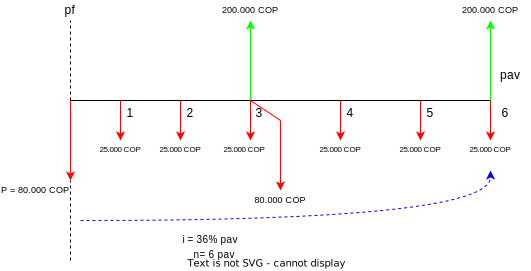
\includegraphics[trim=-5 -5 -5 -5 , scale=0.5,width=150px, height=125px]{9_Capitulo/ejemplos/4/Capitulo9Ejercicio4a.pdf} &  
		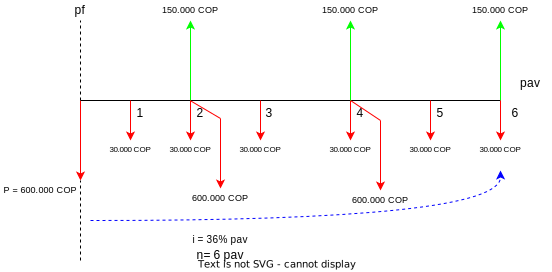
\includegraphics[trim=-5 -5 -5 -5 , scale=0.5,width=150px, height=125px]{9_Capitulo/ejemplos/4/Capitulo9Ejercicio4b.pdf}  \\ \hline
		%%%%%%%%%%%%% FIN INSERCION DE IMAGEN
		%%%%%FIN FLUJO DE CAJA



		%%%%% INICIO DECLARACION FORMULAS
		%%%%%%%%%%% INICIO TITULO
		\rowcolor[HTML]{FFB183}
		\multicolumn{2}{|c|}{\cellcolor[HTML]{FFB183}\textbf{4. Declaración de fórmulas}}    \\ \hline
		%%%%%%%%%%% FIN TITULO
		%%%%%%%%%%% INICIO MATEMATICAS
		\multicolumn{2}{|c|}{$\sum F_{n}(1+i)^{-n} $\hspace{0.3cm} \textit{Valor presente neto}} \\ \hline
		%%%%%%%%%% FIN MATEMATICAS
		%%%%%% INICIO DESARROLLO MATEMATICO
		\rowcolor[HTML]{FFB183}
		%%%%%%%%%%INICIO TITULO
		\multicolumn{2}{|c|}{\cellcolor[HTML]{FFB183}\textbf{5. Desarrollo matemático}}       \\ \hline
		%%%%%%%%%% FIN TITULO
		%%%%%%%%%% INICIO MATEMATICAS
		\multicolumn{2}{|c|}{$VPN_{A} = -800.000-800.000(1+0.36)^{-3}+200.000(1+0.36)^{-3}$}\\
		\multicolumn{2}{|c|}{$-25.000(1+0.36)^{-6} + 200.000(1+0.36)^{-6}$} \\
		\multicolumn{2}{|c|}{$VPN_{A} = -1.065.338 COP$} \\
		\multicolumn{2}{|c|}{$VPN_{B} = -600.000-30.000(\frac{1-((1+0.36)^{-3})}{0.36})$}\\
		\multicolumn{2}{|c|}{$-450.000 (1+0.36)^{-2}-450.000(1+0.36)^{-4}+150.000  1+0.36)^{-6}$} \\
		\multicolumn{2}{|c|}{$VPN_{B} = -1.021.293 COP$} \\ \hline

		%%%%%%%%%% FIN MATEMATICAS
		%%%%%% FIN DESARROLLO MATEMATICO
		%%%%%% INICIO RESPUESTA
		\rowcolor[HTML]{FFB183}
		%%%%%%%%%%INICIO TITULO
		\multicolumn{2}{|c|}{\cellcolor[HTML]{FFB183}\textbf{6. Respuesta}}   \\ \hline
		%%%%%%%%%% FIN TITULO
		%%%%%%%%%% INICIO RESPUESTA MATEMATICA
		\multicolumn{2}{|c|}{Al hacer la compra de la maquina bajo las condiciones dadas en la alternativa II,}  \\
		\multicolumn{2}{|c|}{la empresa tendrá perdidas, sin embargo, se observa que las perdidas son menores} \\
		\multicolumn{2}{|c|}{que al hacer uso de la Alternativa I, así que se escoge la Alternativa II.}  \\ \hline
		%%%%%%%%%% FIN MATEMATICAS
		%%%%%% FIN RESPUESTA
	\end{longtable}
	%Se crean dos lineas en blanco para que no quede el siguiente texto tan pegado
	%\newline \newline %USARLO SI CREES QUE ES NECESARIO
\end{center}
%%%%%%%%%%%%%%%%%%%%%%%%%%FIN EJERCICIO 4 %%%%%%%%%%%%%%%%%%%%%%%%%%%
